\documentclass{article}
\usepackage[utf8]{inputenc}
\usepackage{geometry, parskip, hyperref}
\usepackage{amsfonts, amsmath}
\usepackage{pgfplots, graphicx}
\usepackage{caption, subcaption}


\title{
    \textbf{ECE250: Signals \& Systems} \\
    \large{Assignment 2: Report}
}

\author{\href{mailto:divyajeet21529@iiitd.ac.in}{Divyajeet Singh (2021529)}}

\date{September 30, 2022}

\geometry{a4paper, left=25mm, right=25mm, top=25mm, bottom=25mm}
\pgfplotsset{compat=1.18}

\begin{document}
    \maketitle

    \textbf{Assumptions:}

    \begin{enumerate}
        \item The signal $u(t)$ is the unit-step signal, defined below: \begin{equation}
            u(t) = \begin{cases}
                1 & \text{ if } t \geq 0 \\
                0 & \text{ if } t < 0
            \end{cases}
        \end{equation}
    \end{enumerate}

    \textbf{Question: 1}

    \begin{figure}[h]
        \centering
        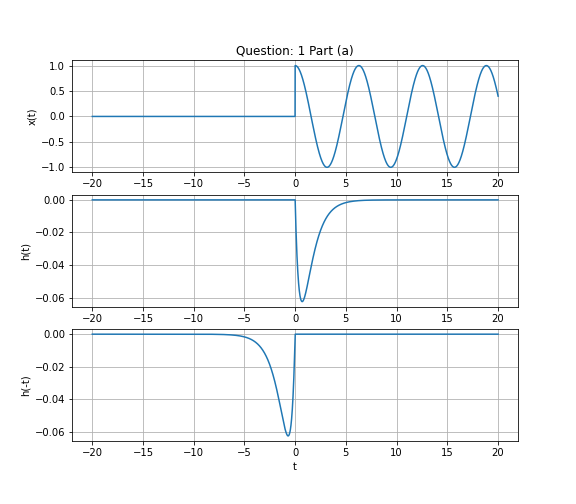
\includegraphics[scale=0.39]{./Assets/1-a-i.png}
        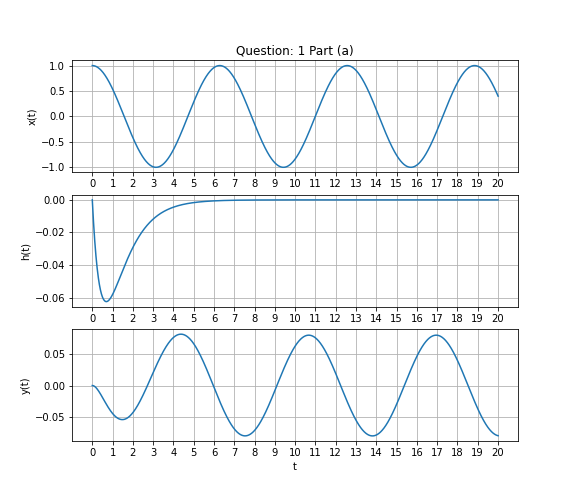
\includegraphics[scale=0.39]{./Assets/1-a-ii.png}
        \caption*{Subplots for \textbf{Question: 1 (a)}}
    \end{figure}

    \begin{figure}[h]
        \centering
        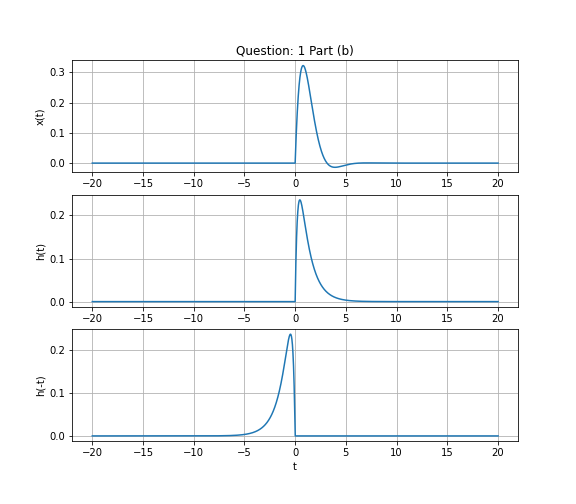
\includegraphics[scale=0.39]{./Assets/1-b-i.png}
        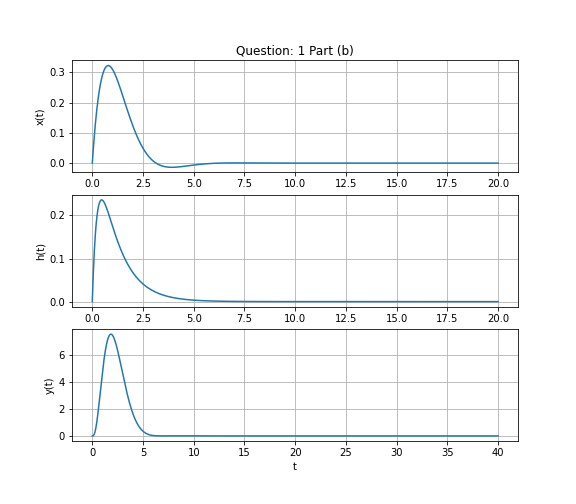
\includegraphics[scale=0.39]{./Assets/1-b-ii.png}
        \caption*{Subplots for \textbf{Question: 1 (b)}}
    \end{figure}


\end{document}